\documentclass[a4paper]{article}
\usepackage[T1]{fontenc}
\usepackage[french]{babel}
\usepackage{hyphenat}
\hyphenation{mate-mática recu-perar}
\usepackage{algpseudocode}
\usepackage{graphicx}
\usepackage{glossaries}
\usepackage[title]{appendix}
\usepackage{listings}
\usepackage{hyperref}

\title{\textit{Travail d'étude et de recherche} \\ \textbf{Apprentissage d'une stratégie d'attaque
contre un véhicule autonome}}
\author{Antoine Roumilhac (20214495@etud.univ-evry.fr) \\ Yara El-Halawani (20235309@etud.univ-evry.fr) \\ encadré·e·s par Guillaume Hutzler \\ en collaboration avec Witold Klaudel, Artur Rataj, \\ Hanna Klaudel, Franck Pommereau}
\date{15 mai 2024}

\renewcommand*\contentsname{Table des matières}
\renewcommand{\refname}{Références}

\graphicspath{ {images/} }

\lstset{
    breaklines=true
}

\begin{document}
    \maketitle

    \vspace*{\fill}

    \begin{center}
        
\includegraphics[height=2cm]{logo_ueve.png}
        
\includegraphics[height=2cm]{logo_ibisc.png}

        
\includegraphics[height=2cm]{logo_systemx.png}
        
\includegraphics[height=2cm]{logo_safetech.png}
    \end{center}

    \newpage

    \section{Introduction}

    \subsection{Contexte du projet}

    Les véhicules autonomes représentent l'une des avancées technologiques les plus prometteuses de notre époque, avec des implications majeures pour la mobilité, la sécurité routière et l'efficacité des transports. Cependant, cette innovation s'accompagne de défis importants, notamment en ce qui concerne la cybersécurité. Les véhicules autonomes dépendent d'une multitude de composants matériels et logiciels, allant des capteurs et des actionneurs aux systèmes d'exploitation et aux algorithmes de prise de décision. Cette complexité technique expose ces systèmes à des risques de cyberattaques, susceptibles de causer des dysfonctionnements graves, voire des accidents.

    Pour garantir la sécurité des véhicules autonomes, il est crucial d'identifier les vulnérabilités potentielles et de mettre en place des mesures de protection efficaces. C'est dans ce contexte que s'inscrit ce projet, qui vise à utiliser des techniques d'apprentissage automatique, et plus précisément des algorithmes de Q-Learning, pour apprendre des stratégies d'attaque efficaces contre un véhicule autonome. L'objectif est de simuler des attaques potentiellement dangereuses afin de détecter les failles de sécurité qui pourraient exister dans ces systèmes.

    Le projet s'appuie sur des travaux antérieurs qui ont modélisé les interactions entre les différents modules d'un véhicule autonome et ont exploré des approches formelles pour analyser les risques de propagation de défaillances. Toutefois, face à la complexité croissante des systèmes de transport intelligents, ces approches peuvent se heurter à des limitations dues à l'ampleur de l'espace d'état à explorer. C'est pourquoi ce projet propose d'adopter des techniques d'apprentissage automatique pour analyser de manière efficace les scénarios d'attaque potentiels.

    \subsection{Objectif du Travail d'étude et de recherche}

    L'objectif de notre projet consiste en une revue des principales variantes d'algorithmes de Q-Learning, en la sélection de la variante la plus adaptée au problème, en la recherche d'une implémentation open source ou le développement d'une nouvelle implémentation, et enfin en l'application de l'algorithme sélectionné à un modèle test.

    \subsection{État de l'art}

    De nombreux travaux ont été produits sur la génération automatique de stratégies d'attaque, par exemple en utilisant des grands modèles de langage \cite{xu_autoattacker_2024} pour faciliter la simulation de cyber-attaques sur des systèmes à sécuriser.
    D'autres approches utilisent la théorie des jeux pour évaluer les risques liés aux cyber-attaques \cite{law_security_2015}.

    Concernant la sécurité pour les véhicules autonomes, d'autres approches sont utilisées.
    On peut voir des approches à base de génération d'arbres d'attaque, qui permettent de ne pas avoir à créer manuellement des stratégies d'attaque \cite{kern_model-based_2021} \cite{sowka_review_2023}.

    Nous n'avons cependant pas trouvé d'article étudiant l'utilisation d'une variante mono-agent simple du Q-Learning dans le cadre de détection préalable de cyber-attaque.

    Il est donc intéressant d'étudier les performances de l'algorithme de Q-Learning sur ce problème.

    \section{Simulation de cyberattaques}

    \subsection{Principe}

    Les cyberattaques posent un défi majeur aux systèmes cyberphysiques, qui sont composés de nombreux éléments variés, souvent employés dans des secteurs critiques, et sont exposés à de multiples cyberattaques. Une cyberattaque consiste en une série d'actions menées par un attaquant, visant à prendre le contrôle de certaines parties du système et lui entraînant des dommages potentiellement importants.

    La détection de ces attaques est essentielle pour améliorer les architectures et les mesures de sécurité, assurant ainsi un niveau de risque tolérable. Par conséquent, il est nécessaire d'évaluer la probabilité des cyberattaques pour estimer le risque global.

    Plusieurs approches pour interpréter la probabilité d’une cyberattaque ont été proposées :

    \begin{itemize}
        \item L'approche des arbres d'attaques \cite{xie_security_2013} : cette approche propose de traduire la probabilité d'une cyberattaque en un coût qui est inversement proportionnel à cette probabilité. Cela permet de calculer le coût total d'une attaque en additionnant les coûts de chaque action qui la compose. Pour modéliser les scénarios d'attaque, nous utilisons souvent des arbres d'attaque qui représentent les chemins possibles qu'un attaquant pourrait emprunter pour compromettre un système, mais la création d'arbres d'attaque est souvent effectuée manuellement par des experts en sécurité, ce qui peut être fastidieux et source d'erreurs.

        \item L’approche des méthodes automatisées \cite{ardito_artificial_2021} : pour rendre ce processus plus efficace, on peut plutôt utiliser des méthodes automatisées. Ces méthodes utilisent des actions atomiques, des étapes spécifiques que des attaquants peuvent utiliser pour compromettre un système. Ces actions représentent des vulnérabilités connues ou des failles zero-day.
    \end{itemize}

    Les langages qui décrivent ces actions atomiques permettent de définir des règles de propagation d'attaques et des conditions pour chaque action. Un problème majeur avec cette approche est le risque d'explosion combinatoire dû à un grand nombre d'actions atomiques possibles. Cela peut rendre les approches manuelles inefficaces, ce qui pousse à limiter le nombre d'actions pour réduire la complexité.

    Ces méthodes automatisées sont souvent meilleures pour auditer des systèmes existants, mais moins utiles pour la conception de nouveaux systèmes, ce qui limite leur pertinence pour choisir les meilleures mesures de cybersécurité.

    \subsection{Approche proposée}

    Le modèle que nous avons sélectionné est décrit dans un rapport technique du laboratoire IBISC de l'Université d'Évry, de l'institut de recherche SystemX et de SafeTech Cybernetics \cite{hutzler_automatic_2024}, et décrit une approche d'estimation de la probabilité de la réalisation d'une cyber-attaque sur un système donné.
    
    Cette approche considère le système comme un ensemble de composants logiciels et matériels. Les composants logiciels exposent des interfaces nécessaires à leur fonctionnement, mais qui peuvent être exploités par des attaquants.
    Le coût d'exploitation de ces interfaces par un attaquant dépend de divers facteurs, tels que la complexité fonctionnelle et les contraintes matérielles.

    \subsubsection{Composants logiciels et matériels du modèle}

    Les composants matériels sont reliés par des liens réseau simples, tandis que les composants logiciels sont connectés par des interactions fonctionnelles dirigées via des protocoles de communication comme HTTP. 
    Chaque composant logiciel est attribué à un composant matériel spécifique. 
    Les composants matériels peuvent être équipés de systèmes d'exploitation ou fonctionner sans. Chaque composant matériel a ses propres règles de routage, déterminant les chemins physiques possibles des interactions. 
    Ces règles sont parfois plus flexibles que nécessaires, offrant des opportunités d'attaque supplémentaires.

    Les éléments essentiels du modèle sont les composants logiciels qui interagissent entre eux selon les règles de propagation de cyber attaques, un attaquant est modélisé par un composant logiciel ayant des privilèges spécifiques.

    \begin{figure}
        \includegraphics[width=\textwidth]{Système.jpg}
        \caption{Exemple d'architecture logicielle et matérielle}
        \label{fig:systeme}
    \end{figure}

    \subsubsection{Modélisation du système}

    La modélisation du système se base sur la construction d'un graphe de visibilité des composants du système.
    Chaque composant logiciel et matériel du système est représenté par un n\oe ud dans le graphe, et chacun des rôles du composant est représenté comme un sous-n\oe ud.
    Ensuite, chaque lien entre les composants est représenté par une arête orientée, partant d'un n\oe ud et terminant sur un rôle d'un autre n\oe ud.
    
    Pour le système de la figure \ref{fig:systeme}, on obtient donc le graphe de la figure \ref{fig:graphe}. Dans cet exemple, on peut voir par exemple que le Hacker voit les rôles 1 et 6, de Routing et HttpSrv respectivement.

    \begin{figure}
        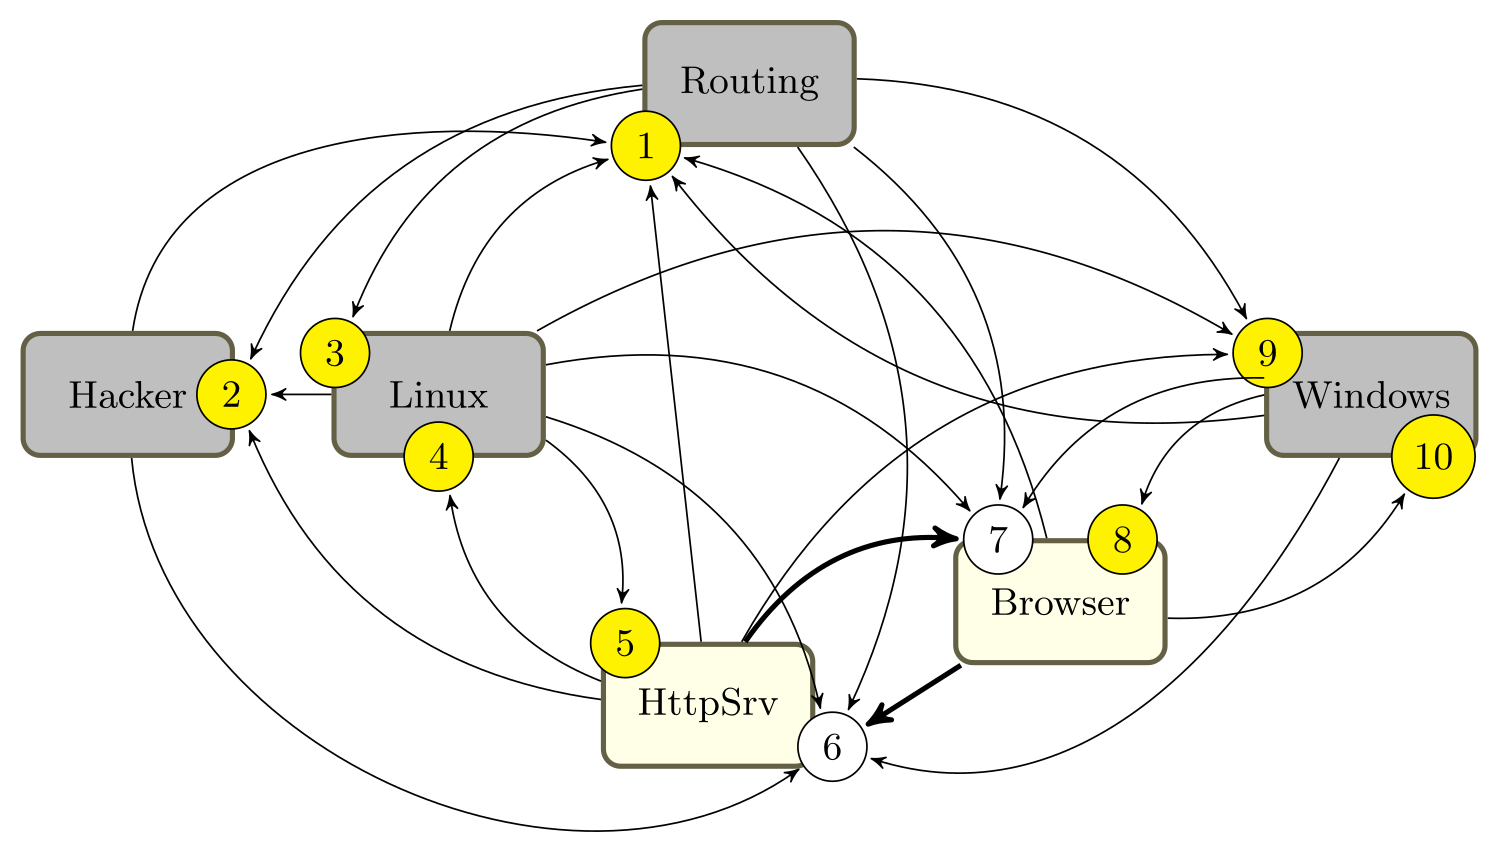
\includegraphics[width=\textwidth]{Graphe.png}
        \caption{Graphe de visibilité du système de la figure \ref{fig:systeme}}
        \label{fig:graphe}
    \end{figure}

    \begin{figure}
        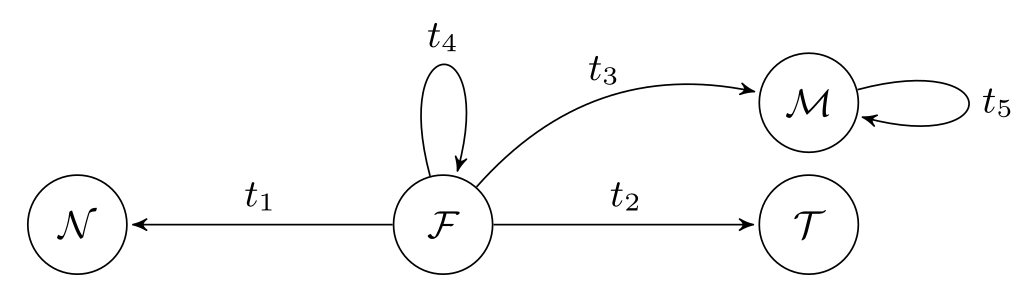
\includegraphics[width=\textwidth]{Automate.png}
        \caption{Automate d'un composant d'un système}
        \label{fig:automate}
    \end{figure}

    Tous les n\oe uds du graphe possèdent un automate, décrit par la figure \ref{fig:automate}, qui décrit son état de fonctionnement actuel.
    Chaque n\oe ud peut être dans l'un des 4 états suivants :

    \begin{itemize}
        \item Fonctionnel (F) : le composant fonctionne normalement.
        \item Données altérées (T) : le composant produit des données de mauvaise qualité pouvant compromettre le fonctionnement des n\oe uds qui dépen-dent de celles-ci. 
        \item Non disponible (N) : le composant n'est plus accessible et ne produit plus de données.
        \item Malware (M) : le composant est infecté par l'attaquant, lui permettant de propager son attaque. Un état Malware peut être interprété comme n'importe quel état par un n\oe ud successeur.
    \end{itemize}

    Chacun des n\oe uds peut contenir des secrets, qui peuvent être volés par l'attaquant.

    Chaque arête du graphe est étiquetée en fonction de la position de l'attaquant dans l'interaction entre les n\oe uds :

    \begin{itemize}
        \item Peer : si le n\oe ud attaquant est un pair fonctionnel dans cette interaction.
        \item MITM : si le n\oe ud se trouve sur un chemin de routage possible pris par l'interaction.
        \item Side : si les règles de routage permettent simplement au n\oe ud attaquant de voir le rôle cible mais que le n\oe ud n'est ni en position peer ou MITM.
    \end{itemize}

    Chaque rôle d'un n\oe ud peut être soit obligatoire, soit optionnel, soit transparent.
    Pour chaque n\oe ud, on définit les variables $thresh_N$ et $thresh_T$.

    Dans chaque automate, il y a 5 transitions entre les états, qui peuvent être réalisées sous certaines conditions :

    \begin{itemize}
        \item F vers N : disponible s'il y a le nombre de n\oe uds pointant vers des rôles optionnels du n\oe ud qui sont non-disponibles est supérieur à $thresh_N$, si l'un des rôles obligatoires du n\oe ud est pointé par un n\oe ud non disponible, ou si l'un de ces n\oe uds est dans l'état Malware.
        \item F vers T : disponible s'il y a le nombre de n\oe uds pointant vers des rôles optionnels du n\oe ud qui sont dans l'état Données altérées est supérieur à $thresh_T$, si l'un des rôles obligatoires du n\oe ud est pointé par un n\oe ud dans l'état Données altérées, ou si l'un de ces n\oe uds est dans l'état Malware.
        \item F vers M : disponible si l'un des n\oe uds pointant vers l'un des rôles du n\oe ud est dans l'état Malware.
        \item F vers F : disponible s'il y a au moins un secret du n\oe ud qui est non volé, et si l'un des n\oe uds pointant vers l'un des rôles du n\oe ud est dans l'état Malware.
        \item M vers M : disponible s'il y a au moins un secret du n\oe ud qui est non volé.
    \end{itemize}

    Chacune de ces transitions a un coût, et la somme des coûts des transitions effectuées donne la difficulté de la stratégie de cyber-attaque.

    \subsubsection{Calcul du coût d'une transition}

    Le coût des transitions dépend de plusieurs variables :
    
    \begin{itemize}
        \item $\kappa_E$ : coût de destruction du protocole de communication entre deux n\oe uds.
        \item $\kappa_R$ : coût d'une injection de code malicieux permettant de forcer le changement de l'état d'un n\oe ud, de la production de données altérées et de vol d'un secret à distance (transition F vers F).
        \item $\kappa_N$ : coût du vol d'un secret quand le n\oe ud est dans l'état Malware.
    \end{itemize}

    Le calcul du coût des transitions est défini précisément dans le code dans l'annexe B.

    \section{Q-Learning}

    Le Q-Learning est un algorithme clé de l'apprentissage par renforcement (RL) qui a évolué pour répondre aux défis de la résolution de problèmes complexes. Initialement conçu comme une approche simple pour les environnements mono-agents, il a ensuite été adapté pour des environnements multi-agents et des applications diversifiées grâce à des variantes.

    \subsection{Principe}

    Il existe différents types d'algorithmes de Q-Learning \cite{jang_Q-Learning_2019} classés en différentes catégories, mais nous nous intéressons d'abord à la variante simple pour un système avec un seul agent.

    On considère un système avec un agent qui peut réaliser certaines actions.
    L'objectif de l'algorithme de Q-Learning est de construire une table, appelée Q-Table, qui reflète quelle est la meilleure action à réaliser pour l'agent en fonction de l'état du système.

    On calcule ainsi pour chaque état $s$ et chaque action $a$ une valeur, appelée Q-Value, qui correspond à la qualité de l'action $a$ quand le système se trouve dans l'état $s$.
    Plus la Q-value est grande, plus l'action est avantageuse à utiliser.

    On initialise la Q-Table avec une certaine valeur, par exemple 0.
    Ensuite, on réalise plusieurs itérations d'entraînement. En partant d'un état initial, l'agent va successivement sélectionner des actions à réaliser, en suivant une politique de choix d'action.
    Par exemple, on pourra définir un paramètre de probabilité d'exploration, et choisir en fonction de cette probabilité entre explorer une action aléatoire parmi celles disponibles, soit sélectionner l'action de Q-value maximale.

    Après chaque choix d'action, on met à jour la Q-value en fonction du résultat de cette action.
    Lorsque, dans l'état $s$, on sélectionne l'action $a$ à réaliser, on passe dans l'état $s'$ et on met à jour la Q-value en utilisant l'équation de Bellman suivante :

    $$ Q^{new}(s,a) \leftarrow Q(s,a) + \alpha [R + \gamma \max Q'(s',a') - Q(s,a)]$$

    Les paramètres de cette fonction sont les suivants :

    \begin{itemize}
        \item $\alpha$ est le taux d'apprentissage, entre 0 et 1.
        \item $R$ est la récompense obtenue en allant dans l'état s'.
        \item $\gamma$ est le facteur d'actualisation (discount factor).
        \item $maxQ(s',a')$ est la valeur Q maximale qu'on peut obtenir à partir de l'état s'.
    \end{itemize}

    L'annexe A résume le fonctionnement de l'algorithme de Q-Learning.

    \subsection{Variantes du Q-Learning}

    La variante de Q-Learning présentée plus haut est relativement simple et convient bien à un environnement à un seul agent.
    Cependant il y a des situations où le système est plus complexe, ou comporte plusieurs agents.
    Pour ces différents cas, d'autres variantes du Q-Learning ont été créées.

    \subsubsection{Variantes mono-agent}

    \begin{itemize}
        \item Deep Q-Learning \cite{liu_deep_2017} : Utilise des réseaux de neurones pour approximer les valeurs d'action. Des techniques comme l'expérience replay et le réseau de cibles contribuent à la stabilité de l'apprentissage.
        \item Q-Learning hiérarchique \cite{junius_ho_hiq_2006} : Divise l'action en niveaux hiérarchiques, accé-lérant le traitement dans des environnements complexes.
        \item Double Q-Learning \cite{hasselt_double_nodate} : Résout le problème de surestimation en utilisant deux fonctions Q distinctes, ce qui réduit le biais.
\end{itemize}

    \subsubsection{Variant multi-agent}

    \begin{itemize}
        \item Modular Q-Learning \cite{ono_multi-agent_1996} : Adapte le Q-Learning à des environnements multi-agents en décomposant les problèmes complexes en sous-problèmes et en les traitant séparément.
        \item Ant Q-Learning \cite{gambardella_ant-q_1995} : Inspiré par le comportement des fourmis, ce modèle utilise des agents coopératifs qui échangent des valeurs AQ, permettant de trouver efficacement des récompenses dans des environnements multi-agents.
        \item Nash Q-Learning \cite{hu_nash_nodate} : L'agent Nash Q-Learning tente d'apprendre ses valeurs Q d'équilibre, en commençant par une supposition arbitraire. À cette fin, l'agent Nash Q-Learning maintient un modèle des valeurs Q des autres agents et utilise cette information pour mettre à jour ses propres valeurs Q.
    \end{itemize}

    \section{Adaptation du problème de calcul de probabilité d'attaque au Q-Learning}

    Après avoir étudié les spécificités du modèle de simulation et d'estimation de coût de cyber-attaques, nous avons réfléchi à l'adaptation de ce modèle pour utiliser le Q-Learning, afin d'apprendre la meilleure stratégie d'attaque sur le système.
    Ensuite, nous avons implémenté le simulateur pour le modèle d'estimation de coût et l'algorithme de Q-Learning.

    \subsection{Choix des états et des actions pour le Q-Learning}

    Pour utiliser l'algorithme de Q-Learning pour notre problème, il est nécessaire de définir quelles sont les états et les actions qui seront utilisées pour la Q-Table.

    Pour les actions, nous pouvons simplement décider de conserver toutes les transitions de tous les automates des composants du système. Cela fait donc un total de $5n$ actions dans notre cas, avec $n$ le nombre de n\oe uds dans le graphe de visibilité.

    Pour le choix des états, le choix est un peu plus complexe.
    En effet, pour des petits systèmes, il peut être envisageable de lister la totalité des états possibles du système, en listant les états de chaque composant du système.
    Cependant, pour de grands systèmes, ce choix n'est pas judicieux car on a alors $5^n$ états possibles, avec $n$ le nombre de n\oe uds du graphe de visibilité, ce qui est un nombre bien trop grand d'états pour entraîner un modèle en un temps raisonnable avec l'algorithme de Q-Learning pour des valeurs grandes de $n$.
    
    Pour des raisons de simplicité et de possibilité d'implémentation, nous avons toutefois choisi de réaliser notre étude avec cet ensemble d'état, mais en gardant un système de petite taille pour que l'exécution de l'algorithme de Q-Learning reste.
    Nous discuterons à la suite des résultats de notre étude des différentes possibilités qui fonctionneraient pour des systèmes de grande taille.

    \subsection{Implémentation d'un simulateur de cyber-attaque}

    Pour les besoins de notre implémentation, nous avions besoin d'avoir un simulateur qui calculerait quelles sont les transitions possibles à chaque état, et également quel est leur coût.

    Nous sommes tout d'abord parti sur la possibilité d'utiliser un simulateur déjà existant.
    Nous avons donc tout d'abord utilisé le logiciel \textit{hyena} \cite{pommereau_fpomhyena_nodate}, réalisé par Franck Pommereau.
    Celui-ci nous permet de spécifier un système que l'on aimerait simuler, à l'aide d'un fichier JSON pour la description du graphe de visibilité et des relations entre les différents n\oe uds du système, et de scripts Python pour définir le comportement des automates de chaque n\oe ud.
    Cependant, nous avons rencontré quelques difficultés lors de l'utilisation de ce logiciel, ce qui nous a poussé à réaliser notre propre simualteur.

    Pour réaliser notre simulateur, nous nous sommes basés sur le modèle Uppaal réalisé pour l'article décrivant l'approche de simulation de cyber-attaques que nous avons sélectionné \cite{hutzler_automatic_2024}.
    Uppaal est un logiciel permettant de modéliser, valider et vérifier des systèmes en temps réel, modélisés comme des réseaux d'automates temporisés \cite{noauthor_httpsuppaalorg_nodate}, c'est à dire des automates qui permettent de rentranscrire des contraintes temporelles en utilisant un ensemble fini de valeurs d'horloge \cite{alur_theory_1994}.
    Pour notre problème, il nous permet de modéliser le système, en définissant un automate par composante du système, et en définissant les gardes de transitions, qui sont les conditions de faisabilité de chaque transition de chaque automate.
    Ces gardes sont définies comme des fonctions programmées dans un langage proche du C.

    Pour réaliser notre simulateur, nous avons donc repris les fonctions et les structures de données définies dans le modèle Uppaal, et nous les avons adaptées en Python.
    Le code que nous avons écrit est disponible dans l'annexe B.
    Nous avons défini les classes Role, pour représenter les rôles de chaque n\oe ud, Input, pour représenter les interactions entre les n\oe uds, Node, pour représenter les n\oe uds, et System, pour représenter l'entièreté du système.

    Ensuite, nous avons défini dans System les méthodes permettant de calculer la faisabilité et le coût des transitions, qui prennent toutes en paramètre l'identifiant du n\oe ud concerné :
    \begin{itemize}
        \item \texttt{System.MinFN} : calcule le coût minimal de la transition de l'état F vers l'état N.
        \item \texttt{System.MinFB} : calcule le coût minimal de la transition l'état F vers l'état B.
        \item \texttt{System.MinFM} : calcule le coût minimal de la transition l'état F vers l'état M.
        \item \texttt{System.RemoteSecrCost} : calcule le coût minimal de la transition l'état F vers l'état F.
        \item \texttt{System.LocalVarCost} : calcule le coût minimal de la transition l'état M vers l'état M.
    \end{itemize}

    Si la transition n'est pas possible, la méthode lui correspondant renvoie la valeur NU, qui est définie à -1 dans notre cas, le coût ne pouvant être négatif.

    La méthode \texttt{computeAvailableTransitions} calcule la liste des transitions qui sont actuellement réalisables, ainsi que leur coût, dans l'état du système actuel.

    Ainsi, avec la liste des transitions disponibles, on peut réaliser un choix pour définir quel sera le prochain état du système, et quel est le coût total de l'attaque.

    Le programme que nous avons réalisé charge le système en utilisant un fichier JSON décrivant les n\oe uds, les interactions et les secrets, d'une manière similaire à ce que fait \textit{hyena}.
    Le fichier JSON que nous avons utilisé pour faire nos essais d'implémentation est donné dans l'annexe C.

    Maintenant que nous avons une implémentation du simulateur de cyber-attaque, on peut implémenter l'algorithme de Q-Learning.

    \subsection{Implémentation de l'algorithme de Q-Learning}

    Pour implémenter l'algorithme de Q-Learning, nous nous sommes basés sur des implémentations simples en Python déjà existantes \cite{noauthor_httpswwwgeeksforgeeksorgQ-Learning--python_2019}.

    On initialise le nombre d'états et d'actions. Pour un sytème à $n$ composants, on a donc $4^n$ états et $5n$ actions dans la Q-Table, qui est donc un tableau de dimension $4^n \times 5n$ et qui est intialisée à 0 au départ, comme sur la figure \ref{fig:qtableinit}.
    Au bout de l'entraînement, on obtient un Q-Table qui est remplie, comme sur la figure \ref{fig:qtablefin}, avec les Q-values qui ont été calculées et qui correspondent bien à la valeur de chaque action à partir de chaque état.

    \begin{figure}[b]
        \centering
        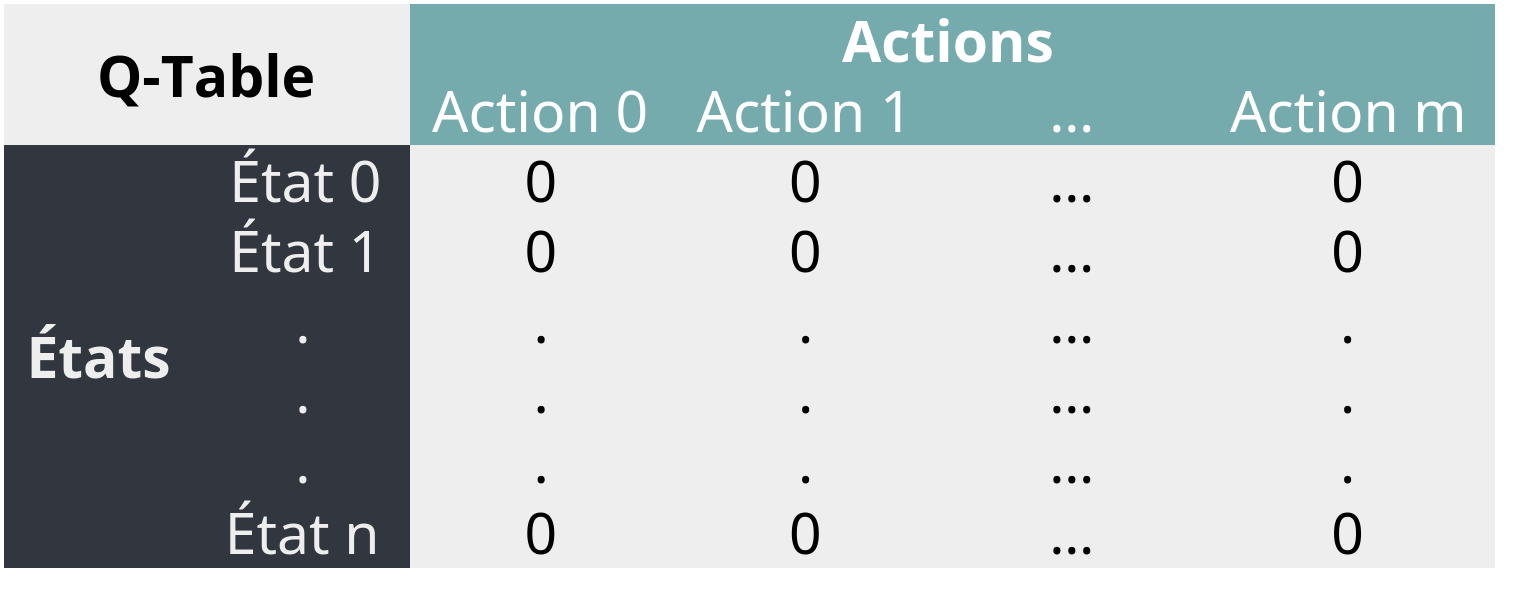
\includegraphics[width=8cm]{QtableInit.png}
        \caption{Initialisation de la Q-Table}
        \label{fig:qtableinit}
    \end{figure}

    \begin{figure}
        \centering
        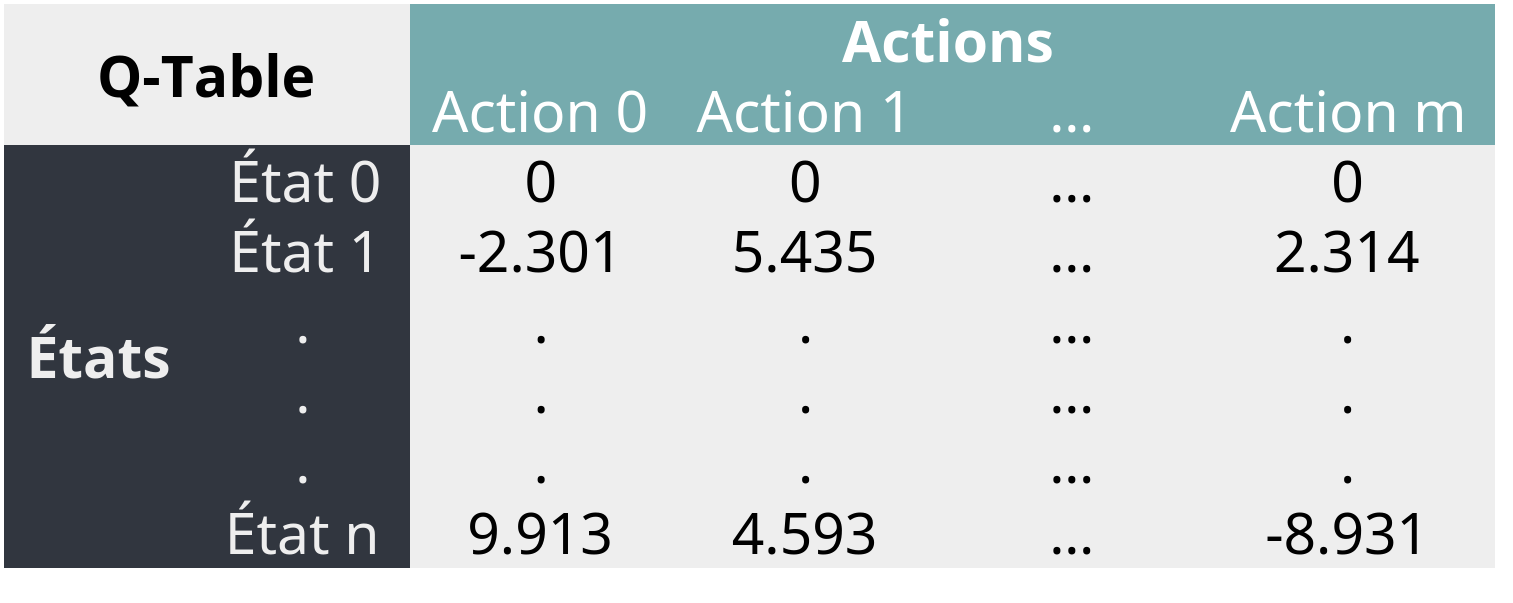
\includegraphics[width=8cm]{QTable2.png}
        \caption{Exemple de Q-Table après l'entraînement}
        \label{fig:qtablefin}
    \end{figure}

    On définit ensuite les différents paramètres de l'algorithme de Q-Learning, à savoir le taux d'apprentissage $\alpha$ et le facteur d'actualisation $\gamma$. 
    Ils prennent tous les deux une valeur réelle entre 0 et 1, et nous verrons dans les résultats quelles sont les meilleures valeurs à leur attribuer.

    On doit également définir la politique de choix d'action que nous voulons utiliser.
    Dans notre cas, nous sommes partis sur l'utilisation d'une politique utilisant un taux d'exploration, qui est la probabilité de choisir une action aléatoire parmi celles disponibles, plutôt que de choisir l'action qui a la Q-value la plus élevée.
    Ainsi, cela permet d'explorer un plus grand nombre d'exécutions différentes, et ainsi d'éviter de tomber dans une exécution qui serait loin d'être optimale sans pouvoir en changer.
    On définit donc, en plus de $\alpha$ et $\gamma$, la variable du taux d'exploration.

    Enfin, on définit le nombre d'itérations à faire pour construire la Q-Table.
    Plus ce nombre est élevé, plus la Q-Table permettra d'avoir l'exécution optimale, mais un nombre trop élevé pourrait compromettre les performances d'apprentissage sans pour autant améliorer les résultats.

    \subsection{Apprentissage et résultats}

    Pour tester notre implémentation, nous allons la tester en utilisant le système décrit par la figure \ref{fig:systeme}, avec le graphe de visibilité décrit par la figure \ref{fig:graphe}.
    Il s'agit d'un système qui est relativement petit, et qui nous permet de tester l'algorithme de Q-Learning sans qu'il y ait trop d'états.

    On commence toujours avec tous les n\oe uds dans l'état Fonctionnel, sauf pour le Hacker qui lui est dans l'état Malware, ce qui lui permet de lancer l'attaque.

    On définit par défaut les paramètres de l'algorithme de Q-Learning aux valeurs suivantes :
    \begin{itemize}
        \item Taux d'apprentissage : $\alpha = 0.8$
        \item Facteur d'actualisation : $\gamma = 0.95$
        \item Taux d'exploration : $\tau = 0.2$
        \item Nombre d'itérations : 10000
    \end{itemize}

    Dans le cas de notre petit exemple, nous n'avons pas de secret à voler, donc on n'en tiendra pas compte ici.

    Concernant la récompense, on va tester deux types de récompenses différentes :
    \begin{itemize}
        \item Donner un score correspondant au nombre de n\oe uds dans un état différent de Fonctionnel.
        \item Donner un score qui est calculé en tenant compte de l'état de chacun des n\oe uds : +1 pour l'état Non disponible, +1.5 pour l'état Données altérées et +2 pour l'état Malware.
    \end{itemize}

    Enfin, pour le coût maximum des attaques, on prend une valeur de 200.
    Chaque itération de l'algorithme de Q-Learning se termine donc soit lorsqu'il n'y a plus de transitions disponibles, soit lorsque le coût total de l'attaque dépasse 200.

    Avec les paramètres par défaut que nous avons définis, et en utilisant la première méthode d'attribution de récompense, on obtient la séquence de transitions suivante :
    \begin{itemize}
        \item Transition de l'état Fonctionnel vers Non disponible du n\oe ud Routing, pour un coût de 50.
        \item Transition de l'état Fonctionnel vers Non disponible du n\oe ud Browser, pour un coût de 0.
    \end{itemize}

    On peut voir que malgré la définition du coût maximum à 200, l'attaque qui est trouvée par l'algorithme de Q-Learning ne coûte que 50, et est donc facilement réalisable pour l'attaquant.
    On a donc trouvé une vulnérabilité de sécurité sur le système.
    On a cependant pas trouvé une séquence qui met tous les n\oe uds dans un état non fonctionnel, puisque 3 n\oe uds sont toujours fonctionnels au final.

    Avec un taux d'apprentissage de 0.5, on obtient la même séquence de transitions.
    Avec un facteur d'actualisation à 0.75, on obtient également la même séquence de transitions.
    Idem en modifiant le taux d'exploration à 0.4, ou en faisant 20000 itérations, ou en changeant la méthode d'attribution des récompenses.

    On voit donc que dans ce cas, modifier les paramètres du Q-Learning n'a que peu d'impact sur le résultat final.
    Cela modifie seulement l'amplitude des Q-values, mais au final le résultat est le même.

    Au niveau des performances de calcul, en faisant 10000 itérations sur un processeur Intel Core i5-7300HQ cadencé à 3.5GHz, le programme met en moyenne 16 secondes pour calculer les valeurs de la Q-Table.

    On peut donc voir que dans le cas d'un petit exemple, avec seulement 6 n\oe uds différents, dont un n\oe ud attaquant, on a pu calculer en quelques secondes une bonne stratégie d'attaque sur le système.
    Toutefois, pour des systèmes plus grands, avec plus de composantes, on aura de nombreux problèmes à calculer une stratégie optimale avec notre implémentation.
    Notamment, le nombre d'états dans lequel peut être le système est très important.

    Pour notre petit exemple, on arrive déjà à un total de 4096 états différents, et 30 actions différentes, soit 122880 valeurs différentes.
    En réalité, le nombre de Q-values réellement à calculer est plus faible, car le nombre de transitions réalisables dans chaque état est limité.
    Mais pour des systèmes avec plus de n\oe uds, même ce nombre de valeurs à calculer va devenir problématique.

    On doit donc réfléchir à d'autres méthodes pour trouver une séquence de transitions optimale pour des systèmes de grande taille.

    \section{Conclusion et pistes d'amélioration}

    \subsection{Conclusion de nos recherches}

    Au cours de projet, nous avons pu découvrir une approche de simulation de cyber-attaque, ainsi que le principe du Q-Learning et les différentes variantes qui existent.
    Nous avons pu ensuite adapter cette approche de simulation pour l'algorithme de Q-Learning mono-agent simple.
    
    Pour l'implémentation, nous avons réalisé un simulateur de cyber-attaque fonctionnel, et l'algorithme de Q-Learning que nous avons implémenté nous a ainsi permis de calculer rapidement un stratégie d'attaque efficace contre un petit système cyber-physique.

    Toutefois, cette approche a de nombreuses limitations, et pour une utilisation dans le cadre d'un système d'un véhicule autonome, il nous faudrait donc changer d'approche.

    \subsection{Limitations de l'algorithme simple de Q-Learning}

    L'utilisation d'une Q-Table pour le Q-Learning limite fortement la taille maximale du système que nous pouvons tester.
    En effet, le nombre d'états différents augmente de manière exponentielle avec la taille du système.

    Aussi, l'algorithme de Q-Learning ne prend pas en compte le coût total des actions à réaliser, et ne cherche donc pas à maximiser ce coût par rapport à la limite qu'on a fixé pour le coût total maximum.
    Par exemple, même lorsque l'on spécifie un coût maximum de 200, on obtient un stratégie coutant seulement 50 qui ne touche que 2 n\oe uds.
    On pourrait obtenir de meilleures stratégies qui ont un coût se rapprochant davantage de 200.

    Ces deux problématiques rendent l'algorithme de Q-Learning que nous avons utilisé peu efficace pour la problématique de départ, à savoir l'utilisation du Q-Learning dans le cadre de l'apprentissage de stratégie d'attaque contre un véhicule autonome.
    Notamment, le système d'un véhicule autonome contient en effet un nombre très important d'états, et il est donc impossible de créer une Q-Table d'une telle taille.
    
    Pour résoudre ce problème, il faut donc changer d'approche, d'abord en étudiant les possibilités en gardant le principe du Q-Learning, et ensuite en regardant d'autres possibilités de calcul de meilleure stratégie.

    \subsection{Approches de Q-Learning différentes}

    Pour résoudre le problème de la taille Q-Table, on pourrait utiliser des méthodes de Q-Learning qui se passent totalement de l'utilisation d'une Q-Table.

    Le Deep Q-Learning \cite{liu_deep_2017} peut être une bonne approche pour se passer d'une Q-Table.
    En effet, le Deep Q-Learning approxime les Q-values en construisant, grâce à un réseau de neurones, une fonction Q.
    Cette fonction Q permet d'estimer la qualité des actions à partir d'un état donné, sans pour autant stocker en permanence la totalité des Q-values.

    On peut également passer d'un système mono-agent à un système multi-agent, et appliquer un algorithme de Q-Learning mutli-agent pour calculer les stratégies.
    Par exemple, on peut considérer un agent pour représenter l'attaquant, et un agent pour représenter la défense du système contre les cyber-attaques, et ensuite considérer le tout comme un jeu à somme nulle \cite{panfili_game-theoretical_2018}, sur lequel on peut appliquer l'algorithme de Q-Learning.

    En dehors du Q-Learning, il existe d'autres méthodes pour résoudre notre problème.

    \subsection{Alternatives au Q-Learning}

    Une première alternative au Q-Learning est le VA-learning \cite{tang_va-learning_2023}, qui est basé sur le calcul d'une fonction Q, comme le Q-Learning, mais qui décompose cette fonction en deux parties : une partie qui est une fonction correspond à la valeur de l'état actuel du système, et une seconde partie qui correspond à l'avantage résiduel de l'action à partir de l'état.
    Le but du VA-learning est d'approximer ces deux fonctions, et ainsi d'approximer la fonction Q.

    Une autre alternative est l'algorithme acteur-critique \cite{konda_actor-critic_nodate}. Le principe de celui est basé sur deux aspects :
    \begin{itemize}
        \item La partie acteur, qui décide pour l'agent de la meilleure action à réaliser. C'est un approximateur de fonction, qui peut être réalisée par un réseau de neurones.
        \item La partie critique, qui évalue l'action réalisée par l'agent. C'est également un approximateur de fonction, qui prend en compte l'état du système et l'action de l'agent, et renvoie la valeur de l'action.
    \end{itemize}

    Il serait donc intéressant d'utiliser l'une des alternatives pour calculer la stratégie optimale d'attaque sur un système de voiture autonome.

    \section{Remerciements}

    Nous tenons à remercier Guillaume Hutzler, notre encadrant pour ce projet, qui nous a énormément aidé et guidé pour mener à bien ces recherches.

    Nous voulons également remercier Franck Pommereau, qui a réalisé le logiciel \textit{hyena} et qui nous a fait une démonstration de son utilisation, ce qui nous a été très utile pour réaliser la simulation des cyber-attaques, et également Hanna et Witold Klaudel, qui nous ont présenté le principe de la modélisation des cyber-attaques que nous avons utilisé dans ce projet.

    \newpage

    \tableofcontents

    \newpage

    \bibliographystyle{unsrt}
    \bibliography{TER.bib}

    \newpage

    \begin{appendices}
        
    \section{Algorigramme de l'algorithme de Q-Learning}

    \begin{center}
        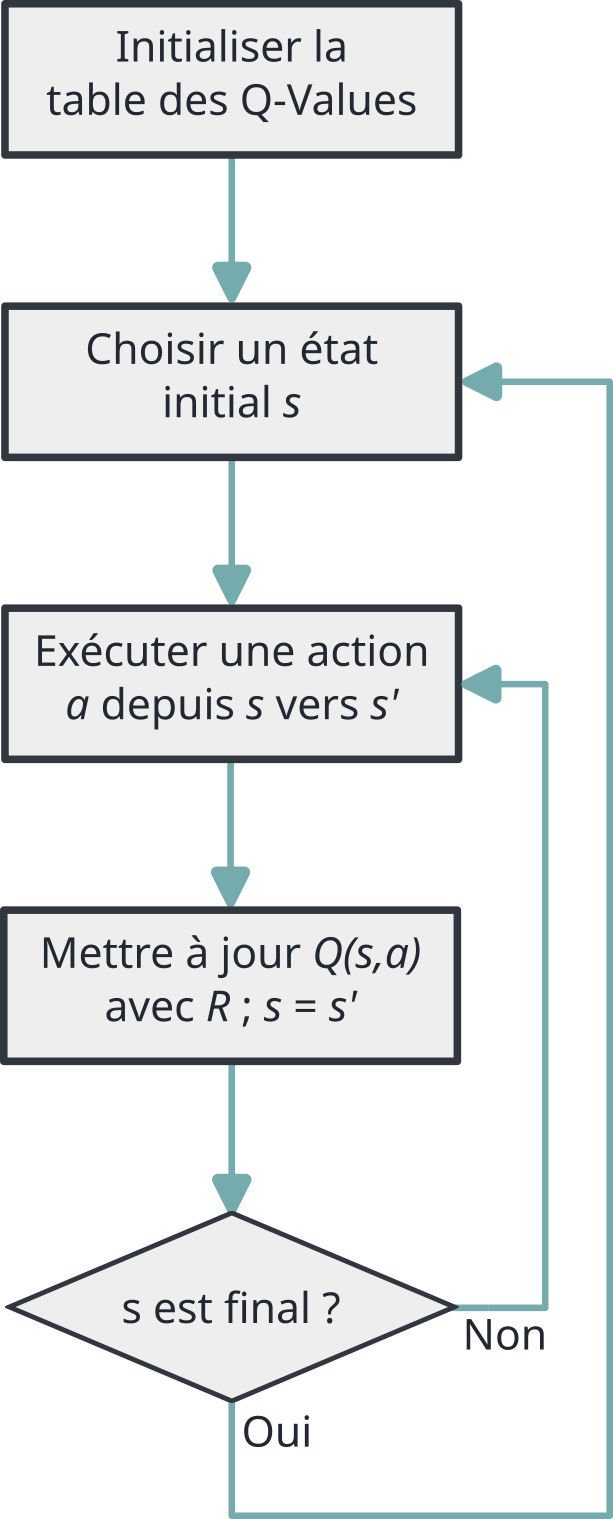
\includegraphics[width=7cm]{algo.png}
    \end{center}

    \newpage

    \section{Code du simulateur de cyber-attaque et de l'algorithme de Q-Learning}

    \begin{lstlisting}[language=python]
import json
import sys
from dataclasses import dataclass
from enum import Enum
import numpy as np

NU = -1

# current : 0 for F, 1 for N, 2 for T, 3 for M
class State(Enum):
    FUNCTIONAL = 0
    NOT_AVAILABLE = 1
    TAINTED = 2
    MALWARE = 3

@dataclass
class Role:
    index: int = 0
    name: str = ""
    protocol: str = ""
    roleType: str = ""
    category: str = ""
    dataBreakCost: int | None = None
    mCodeInjectCost: int | None = None
    bCodeInjectCost: int | None = None
    nCodeInjectCost: int | None = None
    remoteSecrTheftCost = 0
    sessionProtectSecretIndex = []


@dataclass
class Input:
    sourceNodeIndex: int = 0
    debug_sourceNodeName: str = ""
    position: str = ""
    roleIndex: int = 0
    protBreakCostDestruct: int | None = None
    protBreakCostTheft: int | None = None
    protBreakCostTunnelProtocol: int | None = None
    protBreakCostTunnelDecrypt: int | None = None
    protBreakCostTunnelDestroy: int | None = None
    isOpen: str = ""
    tunnelOn: bool = False


@dataclass
class Node:
    current: State = State.FUNCTIONAL
    name: str = ""
    softwareClass: str = ""
    text: str = ""
    kernelIndex: int = 0
    roles = []
    inputs = []
    nodeType: str = ""
    plausThreshold: int = 1
    actThreshold: int = 0
    secrTheftCost: int = 10
    secrStore = []
    monBypassCostToM: int | None = None
    monBypassCostToB: int | None = None
    monBypassCostToN: int | None = None

    def diM(self):
        return len(self.inputs) if len(self.inputs) > 0 else 1

    def diMr(self):
        return len(self.roles) if len(self.roles) > 0 else 1


def minOrNotNone(a, b):
    if a == None:
        return b
    elif b == None:
        return a
    else:
        return min(a, b)

class System:
    nodes: list[Node] = []
    secrets: list[int] = []
    stolenSecrets: list[int] = [False]
    costs = 0
    maxCosts = 200
    nbVar = 0 # Nom de secrets

    def getNodeByName(self, node_name) -> Node:
        for node in self.nodes:
            if node.name == node_name:
                return node
        print(f"Nom de noeud inconnu : {node_name}")
        exit(1)

    def reachable(self, node_id, input_id):
        node = self.nodes[node_id]
        inp: Input = node.inputs[input_id]
        tokens = inp.isOpen.split()

        if len(tokens) <= 0:
            return True
        
        i = 0
        while True:
            if i >= len(tokens):
                print(f"Il manque une expression dans la formule isOpen de l'input {i} du noeud {node.name}")
            i_node_name = tokens[i]
            i_node = self.getNodeByName(i_node_name)
            i+=1
            if i >= len(tokens):
                exit(1)
            if tokens[i] != '<>':
                exit(1)
            i+=1
            if i >= len(tokens):
                exit(1)
            state_str = tokens[i]
            if state_str != '$N':
                exit(1)
            if i_node.current == State.NOT_AVAILABLE:
                return False
            i+=1
            if i >= len(tokens):
                break
            if tokens[i] != '&':
                exit(1)
            i+=1
        return True

    
    def ProtProtectCost(self, node_id: int, input_id: int, role_id: int, sourceNodeIndex: int, attack_position: str) -> int:
        node = self.nodes[node_id]
        protCost: int | None = node.inputs[input_id].protBreakCostTheft
        tunnCost: int | None = node.inputs[input_id].protBreakCostTunnelProtocol
        keyProtect = False
        kernelSId = self.nodes[sourceNodeIndex].kernelIndex

        for i in range(0, self.nbVar - 1):
            if len(node.roles[role_id].sessionProtectSecretIndex) > 0:
                kerSt = False
                if kernelSId != node_id:
                    kerSt = self.nodes[kernelSId].secrStore[i]

                keyProtect = True
                if (self.stolenSecrets[i] or self.nodes[sourceNodeIndex].secrStore[i] or kerSt):
                    protCost = 0

        if attack_position == 'peer':
            if keyProtect:
                if protCost == None:
                    return NU
                return protCost
            else:
                return 0

        if node.inputs[input_id].tunnelOn:
            if protCost == None or tunnCost == None:
                return NU
            else:
                return protCost + tunnCost
        else:
            if protCost == None:
                return NU
            return protCost

    def ProtDestructCost(self, node_id: int, input_id: int, role_id: int, sourceNodeIndex: int, attack_position: str) -> int:
        node = self.nodes[node_id]
        protCostBr = node.inputs[input_id].protBreakCostDestruct
        protCostBr: int = protCostBr if protCostBr != None else NU
        tunCostBr = node.inputs[input_id].protBreakCostTunnelDestroy
        tunCostBr: int = tunCostBr if tunCostBr != None else NU
        keyProtect = False
        protCost = node.inputs[input_id].protBreakCostTheft
        protCost: int = protCost if protCost != None else NU
        tunCost = node.inputs[input_id].protBreakCostTunnelProtocol
        tunCost: int = tunCost if tunCost != None else NU
        kernelSId = node.kernelIndex

        if protCostBr == None or (protCost != None and protCost < protCostBr):
            protCostBr = protCost

        for i in range(0, self.nbVar):
            if len(node.roles[role_id].sessionProtectSecretIndex):
                kerSt = False
                if kernelSId != node_id:
                    kerSt = node.secrStore[i]
                keyProtect = True
                if self.stolenSecrets[i] or self.nodes[sourceNodeIndex].secrStore[i] or kerSt:
                    protCostBr = 0

        if attack_position == 'peer':
            if keyProtect:
                return protCostBr
            else:
                return 0

        if node.inputs[input_id].tunnelOn:
            if tunCost == NU or protCostBr == NU or (tunCost + protCost > tunCostBr):
                return tunCostBr
            return protCostBr + tunCostBr
        else:
            return protCostBr


    def MinCostMalware(self, node_id: int, target_state: State) -> int:
        node = self.nodes[node_id]
        cost = NU
        tcost = NU
        suppl = 0
        if node.nodeType == "kernel" and target_state == State.TAINTED:
            return NU
        if len(node.inputs) <= 0:
            return NU

        for i in range(0, node.diM()):
            if not self.reachable(node_id, i):
                continue
            
            if ((self.nodes[node.inputs[i].sourceNodeIndex].current == State.MALWARE) or (self.nodes[node.inputs[i].sourceNodeIndex].current == State.TAINTED and node.inputs[i].position == 'peer')):
                role_id = node.inputs[i].roleIndex
                role = node.roles[role_id]
                attack_position = node.inputs[i].position
                tcost = self.ProtProtectCost(node_id, i, role_id, node.inputs[i].sourceNodeIndex,attack_position)

                if target_state == State.TAINTED:
                    if tcost > NU and role.bCodeInjectCost != None:
                        tcost += role.bCodeInjectCost
                    else:
                        tcost = NU
                elif target_state == State.NOT_AVAILABLE:
                    if tcost > NU and role.nCodeInjectCost != None:
                        tcost += role.nCodeInjectCost
                    else:
                        tcost = NU
                elif target_state == State.MALWARE:
                    if tcost > NU and role.mCodeInjectCost != None:
                        tcost += role.mCodeInjectCost
                    else:
                        tcost = NU

                if tcost > NU and (cost == NU or tcost < cost):
                    cost = tcost
            
        if cost <= NU:
            return NU

        cost += suppl
        if ((cost + self.costs) <= self.maxCosts):
            return cost
        else:
            return NU


    def minBadDataCost(self, node_id: int):
        node = self.nodes[node_id]
        rolCostBd = [NU] * node.diMr()
        rolOk: list[bool] = [False] * node.diMr()

        bdCost = 0
        tcost = NU
        tr = 0
        totRolOk = 0
        totRolBd = 0
        mustcompromise = NU
        nbCompr = 0
        activityCost = 0
        tr1 = NU
        j = NU

        if len(node.inputs) <= 0:
            return NU
        if node.nodeType == 'kernel':
            return NU

        for i in range(0, node.diM()):
            if self.reachable(node_id, i) and node.roles[node.inputs[i].roleIndex].roleType != 'system' and node.roles[node.inputs[i].roleIndex].category != 'transparent':
                attackerState = self.nodes[node.inputs[i].sourceNodeIndex].current
                role_id = node.inputs[i].roleIndex
                attack_position = node.inputs[i].position
                costDir = node.roles[role_id].dataBreakCost
                protCost = self.ProtProtectCost(node_id, i, role_id, node.inputs[i].sourceNodeIndex, attack_position)
                tt = NU
                if (protCost == NU or costDir == NU):
                    tt = NU
                else:
                    tt += costDir + protCost
                
                if (tt != NU and (attackerState == State.MALWARE) or (attackerState == State.TAINTED and attack_position == 'peer')):
                    if rolCostBd[role_id] == NU or rolCostBd[role_id] > tt:
                        rolCostBd[role_id] = tt

                if attackerState == State.FUNCTIONAL and attack_position == 'peer':
                    rolOk[role_id] = True

        for role_id in range(0, node.diMr()):
            if node.roles[role_id].roleType == 'system':
                continue

            if node.roles[role_id].category == 'mandatory':
                if rolCostBd[role_id] == NU and not rolOk[role_id]:
                    return NU
                if not rolOk[role_id]:
                    mustcompromise = mustcompromise + rolCostBd[role_id] if mustcompromise > NU else rolCostBd[role_id]
                if tcost == NU or rolCostBd[role_id] < tcost:
                    tcost = rolCostBd[role_id]
            elif node.roles[role_id].category == 'optional':
                totRolOk += 1

        if (mustcompromise > NU) and (totRolOk >= node.actThreshold):
            return mustcompromise

        nbCompr = node.actThreshold - totRolOk
        activityCost = 0
        totRolBd = 0
        
        for k in range(0, node.diMr()):
            if nbCompr <= 0:
                continue

            tr1 = NU
            for role_id in range(0, node.diMr()):
                if (node.roles[role_id].roleType != 'system' and node.roles[role_id].category == 'optional' and rolCostBd[role_id] != None and not rolOk[role_id]):
                    if tr1 == NU or tr1 > rolCostBd[role_id]:
                        tr1 = rolCostBd[role_id]
                        j = role_id
            
            if tr1 != NU:
                nbCompr -= 1
                totRolBd += 1
                activityCost += tr1
                rolCostBd[j] = NU
                totRolOk += 1

        if nbCompr > 0:
            return NU

        if mustcompromise > NU:
            return activityCost + mustcompromise

        nbCompr = node.plausThreshold - totRolBd
        bdCost = NU
        for k in range(0, node.diMr()):
            if nbCompr <= 0:
                continue
            tr1 = NU
            for role_id in range(0, node.diMr()):
                if node.roles[role_id].roleType != 'system' and node.roles[role_id].category == 'optional' and rolCostBd[role_id] and rolOk[role_id]:
                    if tr1 == NU or tr1 > rolCostBd[role_id]:
                        tr1 = rolCostBd[role_id]
                        j = role_id
            if tr1 != NU:
                nbCompr -= 1
                if bdCost != NU:
                    bdCost += tr1
                else:
                    bdCost = tr1
                rolCostBd[j] = NU
        
        if nbCompr > 0 and tcost < 0:
            return NU

        if tcost < 0:
            if bdCost < 0:
                return activityCost
            return activityCost + bdCost

        if bdCost != NU:
            return activityCost + (tcost if tcost < bdCost else bdCost)
        return activityCost + tcost


    def BadData(self, node_id: int):
        suppl = 0
        badDataCost = self.minBadDataCost(node_id)
        if badDataCost == NU:
            return NU
        badDataCost += suppl
        if ((badDataCost + self.costs) <= self.maxCosts):
            return badDataCost
        return NU


    def MinFB(self, node_id: int):
        mal = self.MinCostMalware(node_id, State.TAINTED)
        bd = self.BadData(node_id)
        if mal == NU:
            return bd
        if bd == NU:
            return mal
        if bd > mal:
            return mal
        return bd

    def minNonDispCost(self, node_id: int) -> int:
        node = self.nodes[node_id]
        rolCostBdM = [NU] * node.diMr()
        rolOk = [False] * node.diMr()
        nbOKnMand = 0
        tcost = NU
        nbtocomp = 0
        bdCost = NU
        tr = NU

        if len(node.inputs) <= 0:
            return NU

        for input_id in range(0, node.diM()):
            if self.reachable(node_id, input_id) and (node.roles[node.inputs[input_id].roleIndex].category != 'transparent') and (node.roles[node.inputs[input_id].roleIndex].roleType != 'system'):
                attackerState = self.nodes[node.inputs[input_id].sourceNodeIndex].current
                role_id = node.inputs[input_id].roleIndex
                attack_position = node.inputs[input_id].position
                sessDestruct = NU

                if (attackerState == State.FUNCTIONAL) and (attack_position == 'peer'): 
                    rolOk[role_id] = True

                if rolCostBdM[role_id] != 0:
                    sessDestruct = self.ProtDestructCost(node_id, input_id, role_id, node.inputs[input_id].sourceNodeIndex, attack_position)
                    if sessDestruct != NU:
                        if rolCostBdM[role_id] == NU:
                            rolCostBdM[role_id] = sessDestruct
                        elif sessDestruct < rolCostBdM[role_id]:
                            rolCostBdM[role_id] = sessDestruct 

        for role_id in range(0, node.diMr()):
            if node.roles[role_id].roleType != 'system' and node.roles[role_id].category != 'transparent':
                if node.roles[role_id].category == 'mandatory':
                    if not rolOk[role_id]:
                        return 0
                    if rolCostBdM[role_id] != NU:
                        if (tcost == NU) or (rolCostBdM[role_id] < tcost):
                            tcost = rolCostBdM[role_id]
                elif node.roles[role_id].category == 'optional':
                    if rolOk[role_id]:
                        nbOKnMand += 1

        if nbOKnMand < node.actThreshold:
            return 0

        nbtocomp = 1 + nbOKnMand - node.actThreshold

        for k in range(0, node.diMr()):
            tr1 = NU
            j = NU
            
            for role_id in range(0, node.diMr()):
                if node.roles[role_id].roleType != 'system' and node.roles[role_id].category == 'optional' and rolCostBdM[role_id] != NU and tr < nbtocomp:
                    if (tr1 == NU) or tr1 > rolCostBdM[role_id]:
                        tr1 = rolCostBdM[role_id]
                        j = role_id

            if tr1 != NU:
                tr += 1
                bdCost = (bdCost if (bdCost != NU) else 0) + tr1
                rolCostBdM[j] = NU

        if tr < nbtocomp:
            return tcost

        if tcost == NU:
            return bdCost

        return tcost if (bdCost > tcost) else bdCost

    
    def NoProducerDisp(self, node_id: int):
        suppl = 0
        NoProducerDispCost = self.minNonDispCost(node_id)
        if NoProducerDispCost == NU:
            return NU
        NoProducerDispCost += suppl
        if (NoProducerDispCost + self.costs) <= self.maxCosts:
            return NoProducerDispCost
        return NU

    def MinFN(self, node_id: int) -> int:
        node = self.nodes[node_id]
        mal = self.MinCostMalware(node_id, State.NOT_AVAILABLE)
        noProd = self.NoProducerDisp(node_id)

        if mal == NU:
            return noProd
        if noProd == NU:
            return mal
        if noProd > mal:
            return mal
        return noProd

    def MinFM(self, node_id: int) -> int:
        return self.MinCostMalware(node_id, State.MALWARE)
    
    def RemoteSecrCost(self, node_id: int) -> int:
        node = self.nodes[node_id]
        cost = NU
        tcost = NU
        z = 0
        if len(node.inputs) <= 0:
            return NU
        for i in range(0, self.nbVar):
            if (not self.stolenSecrets[i]) and node.secrStore[i]:
                z+=1
        if z == 0:
            return NU
        
        for i in range(0, node.diM()):
            if self.reachable(node_id, i):
                if self.nodes[node.inputs[i].sourceNodeIndex].current == State.MALWARE:
                    role_id = node.inputs[i].roleIndex
                    attack_position = node.inputs[i].position
                    tcost = self.ProtProtectCost(node_id, i, role_id, node.inputs[i].sourceNodeIndex, attack_position)
                    if tcost > NU and node.roles[role_id].remoteSecrTheftCost != None:
                        tcost += node.roles[role_id].remoteSecrTheftCost
                    else:
                        tcost = NU
                    if tcost > NU:
                        if cost == NU or tcost < cost:
                            cost += tcost

        if cost <= NU:
            return NU
        if cost + self.costs <= self.maxCosts:
            return cost
        else:
            return NU
        
    def setRemoteSecr(self, node_id: int):
        node = self.nodes[node_id]
        for i in range(0, self.nbVar):
            if not self.stolenSecrets[i] and node.secrStore[i]:
                self.stolenSecrets[i] = True


    def LocalVarCost(self, node_id: int):
        node = self.nodes[node_id]
        cost = NU
        for i in range(0, self.nbVar):
            if not self.stolenSecrets[i] and node.secrStore[i]:
                cost = node.secrTheftCost
                if (cost + self.costs) <= self.maxCosts:
                    return cost
                return NU

        return NU

    def setLocalSecr(self, node_id: int):
        node = self.nodes[node_id]
        for i in range(0, self.nbVar):
            if not self.stolenSecrets[i] and node.secrStore[i]:
                self.stolenSecrets[i] = True


    def computeAvailableTransitions(self):
        trans = []

        for node_id in range(0, len(self.nodes)):
            node = self.nodes[node_id]

            if node.current == State.FUNCTIONAL:
                fn = self.MinFN(node_id)
                if fn != NU:
                    trans.append((node_id, State.FUNCTIONAL, State.NOT_AVAILABLE, fn, None))

                ft = self.MinFB(node_id)
                if ft != NU:
                    trans.append((node_id, State.FUNCTIONAL, State.NOT_AVAILABLE, ft, None))

                fm = self.MinFM(node_id)
                if fm != NU:
                    trans.append((node_id, State.FUNCTIONAL, State.MALWARE, fm, None))

                ff = self.RemoteSecrCost(node_id)
                if ff != NU:
                    trans.append((node_id, State.FUNCTIONAL, State.FUNCTIONAL, ff, self.setRemoteSecr))

            elif node.current == State.MALWARE:
                mm = self.LocalVarCost(node_id)
                if mm != NU:
                    trans.append((node_id, State.MALWARE, State.MALWARE, mm, self.setLocalSecr))
            
        return trans


def loadSystemFromJSON(file_name: str):
    f = open(file_name)

    data = json.load(f)

    system = System()

    system.nbVar = data['nbSecrets']
    system.stolenSecrets = [False] * system.nbVar

    for n in data['nodes']:
        node = Node()

        node.current = State(n['current'] if ('current' in n) else 0)
        node.name = n['name']
        node.softwareClass = n['softwareClass']
        node.text = n['text']
        node.kernelIndex = n['kernelIndex']
        node.nodeType = n['nodeType']
        node.secrStore = n['secrStore']
        if len(node.secrStore) != system.nbVar:
            node.secrStore = [False] * system.nbVar
        node.monBypassCostToM = n['monBypassCost']['toM']
        node.monBypassCostToB = n['monBypassCost']['toB']
        node.monBypassCostToN = n['monBypassCost']['toN']

        node.roles = []

        roleIndex = 0
        
        for r in n['roles']:
            role = Role(index=roleIndex, name=r['name'], protocol=r['protocol'], roleType=r['type'],
                        category=r['categ'])

            role.dataBreakCost = r['dataBreakCost']
            role.mCodeInjectCost = r['mCodeInjectCost']
            role.bCodeInjectCost = r['bCodeInjectCost']
            role.nCodeInjectCost = r['nCodeInjectCost']
            role.remoteSecrTheftCost = r['remoteSecrTheftCost']
            role.sessionProtectSecretIndex = r['sessionProtectSecretIndex']

            node.roles.append(role)

            roleIndex += 1

        node.inputs = []

        for i in n['inputs']:
            input = Input(sourceNodeIndex=i['sourceNodeIndex'], debug_sourceNodeName=i['debug_sourceNodeName'],
                            position=i['position'], roleIndex=i['roleIndex'], isOpen=i['isOpen'])

            input.protBreakCostDestruct = i['protBreakCosts']['destruct']
            input.protBreakCostTheft = i['protBreakCosts']['theft']
            input.protBreakCostTunnelProtocol = i['protBreakCosts']['tunnelProtocol']
            input.protBreakCostTunnelDecrypt = i['protBreakCosts']['tunnelDecrypt']
            input.protBreakCostTunnelDestroy = i['protBreakCosts']['tunnelDestroy']

            node.inputs.append(input)

        node.plausThreshold = n['plausThreshold']
        node.actThreshold = n['actThreshold']
        node.secrTheftCost = n['secrTheftCost']
        node.secrStore = n['secrStore']

        system.nodes.append(node)

    return system


def calculateReward(system: System):
    score = 0 
    for node in system.nodes:
        if node.current == State.NOT_AVAILABLE:
            score += 1
        elif node.current == State.TAINTED:
            score += 1.5
        elif node.current == State.MALWARE:
            score += 2

    return score


def encodeState(system: System):
    sid = 0
    for i, node in enumerate(system.nodes):
        if node.current == State.TAINTED:
            sid += 1 * (4 ** i)
        elif node.current == State.NOT_AVAILABLE:
            sid += 2 * (4 ** i)
        elif node.current == State.MALWARE:
            sid += 3 * (4 ** i)
    return sid

def encodeAction(transition):
    node_index = transition[0]
    if transition[1] == State.FUNCTIONAL: # curr_state == F 
        if transition[2] == State.FUNCTIONAL: # FF 
            return 5 * node_index
        elif transition[2] == State.TAINTED:
            return 1 + (5 * node_index)
        elif transition[2] == State.NOT_AVAILABLE:
            return 2 + (5 * node_index)
        elif transition[2] == State.MALWARE:
            return 3 + (5 * node_index)
    elif transition[1] == State.MALWARE:
        if transition[2] == State.MALWARE:
            return 4 + (5 * node_index)
        
    pass
    
import copy

def q_learn(initial_state: System, max_cost = 150, learning_rate = 0.8, discount_factor = 0.95, exploration_prob = 0.2, epochs = 10000):
    n_states = 4 ** len(initial_state.nodes)
    n_actions = 5 * len(initial_state.nodes)

    Q_table = np.zeros((n_states, n_actions))

    for epoch in range(epochs):
        current_state = copy.deepcopy(initial_state)
        current_state.nodes = copy.deepcopy(initial_state.nodes)
        current_state.secrets = copy.deepcopy(initial_state.secrets)
        current_state.stolenSecrets = copy.deepcopy(initial_state.stolenSecrets)
        cost = 0
        chosenActions = []

        while cost <= max_cost:        
            sid = encodeState(current_state)

            availableTransitions = current_state.computeAvailableTransitions()
            
            if len(availableTransitions) == 0:
                break

            encodedActions = []

            for trans in availableTransitions:
                encodedActions.append(encodeAction(trans))

            action = 0
            max_action = 0
            max_qvalue = Q_table[sid][encodedActions[0]]

            if np.random.rand() < exploration_prob:
                action = np.random.randint(0, len(availableTransitions))
            else:
                for i, encodedAction in enumerate(encodedActions):
                    q_val = Q_table[sid][encodedAction]
                    if max_qvalue > q_val:
                        max_qvalue = q_val 
                        max_action = i
                action = max_action
            
            chosenAction = availableTransitions[action]
            chosenActions.append(chosenAction)
            current_state.nodes[chosenAction[0]].current = chosenAction[2]
            cost += chosenAction[3]
            if chosenAction[4] != None:
                chosenAction[4](chosenAction[0])

            reward = calculateReward(current_state)

            Q_table[sid,encodedActions[action]] += learning_rate * (reward + discount_factor * np.max(Q_table[encodeState(current_state)]) - Q_table[sid,encodedActions[action]])

    return Q_table

def printBestStrategy(initial_state: System, Q_table: np.array, max_cost: int = 150):
    cost = 0

    current_state = copy.deepcopy(initial_state)
    current_state.nodes = copy.deepcopy(initial_state.nodes)
    current_state.secrets = copy.deepcopy(initial_state.secrets)
    current_state.stolenSecrets = copy.deepcopy(initial_state.stolenSecrets)

    while cost < max_cost:
        cost = 0

        sid = encodeState(current_state)

        availableTransitions = current_state.computeAvailableTransitions()

        if len(availableTransitions) == 0:
            break

        encodedActions = []

        for trans in availableTransitions:
            encodedActions.append(encodeAction(trans))

        max_action = 0
        max_qvalue = Q_table[sid][encodedActions[0]]

        for i, encodedAction in enumerate(encodedActions):
            q_val = Q_table[sid][encodedAction]
            print(q_val)
            if max_qvalue > q_val:
                max_qvalue = q_val 
                max_action = i

        chosenAction = availableTransitions[max_action]
        current_state.nodes[chosenAction[0]].current = chosenAction[2]
        cost += chosenAction[3]
        if chosenAction[4] != None:
            chosenAction[4](chosenAction[0])

        print(current_state.nodes[chosenAction[0]].name, chosenAction[1], chosenAction[2], chosenAction[3])
        
if __name__ == "__main__":
    if len(sys.argv) < 2:
        print("Usage : python3 main.py FICHIER_JSON")
        exit(0)
    system: System = loadSystemFromJSON(sys.argv[1])
    totalCost: int = 0

    q_table = q_learn(system)

    printBestStrategy(system, q_table)

    exit(0)
    \end{lstlisting}

    Fichier \texttt{main.py} disponible à l'url : 
    
    {\centering \href{https://gist.github.com/YoshiLeLama/582b45b0c05ccae4fa71fd3106012f85}{https://gist.github.com/YoshiLeLama/582b45b0c05ccae4fa71fd3106012f85}}

    \newpage

    \section{Fichier JSON décrivant le système}

    \begin{lstlisting}
{
  "nbNodes" : 6,
  "nbSecrets" : 0,
  "secrets" : [ ],
  "nodes" : [ {
    "current":0,
    "name" : "Browser",
    "softwareClass" : "RichBrowser",
    "text" : "Intranet Browser",
    "kernelIndex" : 5,
    "nbRoles" : 3,
    "nbInputs" : 5,
    "nodeType" : "user",
    "plausThreshold" : 1,
    "actThreshold" : 0,
    "secrTheftCost" : 10,
    "secrStore" : [ ],
    "monBypassCost" : {
      "toM" : null,
      "toB" : null,
      "toN" : null
    },
    "roles" : [ {
      "name" : "client",
      "protocol" : "https",
      "type" : "functional",
      "categ" : "mandatory",
      "dataBreakCost" : 5,
      "mCodeInjectCost" : 25,
      "bCodeInjectCost" : 20,
      "nCodeInjectCost" : 15,
      "remoteSecrTheftCost" : 20,
      "sessionProtectSecretIndex" : [ ]
    }, {
      "name" : "x/app",
      "protocol" : "x/WindowsDesktop",
      "type" : "system",
      "categ" : "mandatory",
      "dataBreakCost" : null,
      "mCodeInjectCost" : 20,
      "bCodeInjectCost" : null,
      "nCodeInjectCost" : 1,
      "remoteSecrTheftCost" : 10,
      "sessionProtectSecretIndex" : [ ]
    }, {
      "name" : "x/kernel",
      "protocol" : "x/WindowsDesktop",
      "type" : "system",
      "categ" : "mandatory",
      "dataBreakCost" : null,
      "mCodeInjectCost" : 10,
      "bCodeInjectCost" : null,
      "nCodeInjectCost" : 1,
      "remoteSecrTheftCost" : 10,
      "sessionProtectSecretIndex" : [ ]
    } ],
    "inputs" : [ {
      "sourceNodeIndex" : 2,
      "debug_sourceNodeName" : "HttpSrv",
      "position" : "peer",
      "roleIndex" : 0,
      "protBreakCosts" : {
        "destruct" : 0,
        "theft" : 25,
        "tunnelProtocol" : null,
        "tunnelDecrypt" : null,
        "tunnelDestroy" : null
      },
      "isOpen" : "Windows <> $N & Routing <> $N & Linux <> $N"
    }, {
      "sourceNodeIndex" : 3,
      "debug_sourceNodeName" : "Linux",
      "position" : "mitm",
      "roleIndex" : 0,
      "protBreakCosts" : {
        "destruct" : 0,
        "theft" : 25,
        "tunnelProtocol" : null,
        "tunnelDecrypt" : null,
        "tunnelDestroy" : null
      },
      "isOpen" : "Windows <> $N & Routing <> $N & Linux <> $N"
    }, {
      "sourceNodeIndex" : 4,
      "debug_sourceNodeName" : "Routing",
      "position" : "mitm",
      "roleIndex" : 0,
      "protBreakCosts" : {
        "destruct" : 0,
        "theft" : 25,
        "tunnelProtocol" : null,
        "tunnelDecrypt" : null,
        "tunnelDestroy" : null
      },
      "isOpen" : "Windows <> $N & Routing <> $N"
    }, {
      "sourceNodeIndex" : 5,
      "debug_sourceNodeName" : "Windows",
      "position" : "mitm",
      "roleIndex" : 0,
      "protBreakCosts" : {
        "destruct" : 0,
        "theft" : 25,
        "tunnelProtocol" : null,
        "tunnelDecrypt" : null,
        "tunnelDestroy" : null
      },
      "isOpen" : "Windows <> $N"
    }, {
      "sourceNodeIndex" : 5,
      "debug_sourceNodeName" : "Windows",
      "position" : "peer",
      "roleIndex" : 2,
      "protBreakCosts" : {
        "destruct" : null,
        "theft" : 0,
        "tunnelProtocol" : null,
        "tunnelDecrypt" : null,
        "tunnelDestroy" : null
      },
      "isOpen" : "Windows <> $N"
    } ],
    "fallbackActionIndex" : {
      "toM" : null,
      "toB" : null,
      "toN" : null
    },
    "debug_fallbackActionNames" : "null,null,null"
  }, {
    "current":3,
    "name" : "Hacker",
    "softwareClass" : "Linux",
    "text" : "Hacker Kernel",
    "kernelIndex" : 1,
    "nbRoles" : 3,
    "nbInputs" : 3,
    "nodeType" : "kernel",
    "plausThreshold" : 1,
    "actThreshold" : 0,
    "secrTheftCost" : 10,
    "secrStore" : [ ],
    "monBypassCost" : {
      "toM" : null,
      "toB" : null,
      "toN" : null
    },
    "roles" : [ {
      "name" : "x/user",
      "protocol" : "x/Linux",
      "type" : "system",
      "categ" : "mandatory",
      "dataBreakCost" : null,
      "mCodeInjectCost" : 60,
      "bCodeInjectCost" : null,
      "nCodeInjectCost" : 50,
      "remoteSecrTheftCost" : 50,
      "sessionProtectSecretIndex" : [ ]
    }, {
      "name" : "x/root",
      "protocol" : "x/Linux",
      "type" : "system",
      "categ" : "mandatory",
      "dataBreakCost" : null,
      "mCodeInjectCost" : 20,
      "bCodeInjectCost" : null,
      "nCodeInjectCost" : 10,
      "remoteSecrTheftCost" : 10,
      "sessionProtectSecretIndex" : [ ]
    }, {
      "name" : "x/network",
      "protocol" : "x/Linux",
      "type" : "system",
      "categ" : "mandatory",
      "dataBreakCost" : null,
      "mCodeInjectCost" : 60,
      "bCodeInjectCost" : null,
      "nCodeInjectCost" : 50,
      "remoteSecrTheftCost" : 50,
      "sessionProtectSecretIndex" : [ ]
    } ],
    "inputs" : [ {
      "sourceNodeIndex" : 2,
      "debug_sourceNodeName" : "HttpSrv",
      "position" : "peer",
      "roleIndex" : 2,
      "protBreakCosts" : {
        "destruct" : null,
        "theft" : 0,
        "tunnelProtocol" : null,
        "tunnelDecrypt" : null,
        "tunnelDestroy" : null
      },
      "isOpen" : "Hacker <> $N & Routing <> $N & Linux <> $N"
    }, {
      "sourceNodeIndex" : 3,
      "debug_sourceNodeName" : "Linux",
      "position" : "peer",
      "roleIndex" : 2,
      "protBreakCosts" : {
        "destruct" : null,
        "theft" : 0,
        "tunnelProtocol" : null,
        "tunnelDecrypt" : null,
        "tunnelDestroy" : null
      },
      "isOpen" : "Hacker <> $N & Routing <> $N & Linux <> $N"
    }, {
      "sourceNodeIndex" : 4,
      "debug_sourceNodeName" : "Routing",
      "position" : "peer",
      "roleIndex" : 2,
      "protBreakCosts" : {
        "destruct" : null,
        "theft" : 0,
        "tunnelProtocol" : null,
        "tunnelDecrypt" : null,
        "tunnelDestroy" : null
      },
      "isOpen" : "Hacker <> $N & Routing <> $N"
    } ],
    "fallbackActionIndex" : {
      "toM" : null,
      "toB" : null,
      "toN" : null
    },
    "debug_fallbackActionNames" : "null,null,null"
  }, {
    "current": 0,
    "name" : "HttpSrv",
    "softwareClass" : "WebApp",
    "text" : "Server Htttp",
    "kernelIndex" : 3,
    "nbRoles" : 3,
    "nbInputs" : 6,
    "nodeType" : "user",
    "plausThreshold" : 1,
    "actThreshold" : 0,
    "secrTheftCost" : 10,
    "secrStore" : [ ],
    "monBypassCost" : {
      "toM" : null,
      "toB" : null,
      "toN" : null
    },
    "roles" : [ {
      "name" : "server",
      "protocol" : "https",
      "type" : "functional",
      "categ" : "transparent",
      "dataBreakCost" : 5,
      "mCodeInjectCost" : 25,
      "bCodeInjectCost" : 20,
      "nCodeInjectCost" : 15,
      "remoteSecrTheftCost" : 20,
      "sessionProtectSecretIndex" : [ ]
    }, {
      "name" : "x/app",
      "protocol" : "x/Linux",
      "type" : "system",
      "categ" : "mandatory",
      "dataBreakCost" : null,
      "mCodeInjectCost" : 20,
      "bCodeInjectCost" : null,
      "nCodeInjectCost" : 1,
      "remoteSecrTheftCost" : 10,
      "sessionProtectSecretIndex" : [ ]
    }, {
      "name" : "x/kernel",
      "protocol" : "x/Linux",
      "type" : "system",
      "categ" : "mandatory",
      "dataBreakCost" : null,
      "mCodeInjectCost" : 10,
      "bCodeInjectCost" : null,
      "nCodeInjectCost" : 1,
      "remoteSecrTheftCost" : 10,
      "sessionProtectSecretIndex" : [ ]
    } ],
    "inputs" : [ {
      "sourceNodeIndex" : 0,
      "debug_sourceNodeName" : "Browser",
      "position" : "peer",
      "roleIndex" : 0,
      "protBreakCosts" : {
        "destruct" : 0,
        "theft" : 25,
        "tunnelProtocol" : null,
        "tunnelDecrypt" : null,
        "tunnelDestroy" : null
      },
      "isOpen" : "Linux <> $N & Routing <> $N & Windows <> $N"
    }, {
      "sourceNodeIndex" : 1,
      "debug_sourceNodeName" : "Hacker",
      "position" : "side",
      "roleIndex" : 0,
      "protBreakCosts" : {
        "destruct" : 15,
        "theft" : 25,
        "tunnelProtocol" : null,
        "tunnelDecrypt" : null,
        "tunnelDestroy" : null
      },
      "isOpen" : "Linux <> $N & Routing <> $N & Hacker <> $N"
    }, {
      "sourceNodeIndex" : 3,
      "debug_sourceNodeName" : "Linux",
      "position" : "mitm",
      "roleIndex" : 0,
      "protBreakCosts" : {
        "destruct" : 0,
        "theft" : 25,
        "tunnelProtocol" : null,
        "tunnelDecrypt" : null,
        "tunnelDestroy" : null
      },
      "isOpen" : "Linux <> $N"
    }, {
      "sourceNodeIndex" : 4,
      "debug_sourceNodeName" : "Routing",
      "position" : "mitm",
      "roleIndex" : 0,
      "protBreakCosts" : {
        "destruct" : 0,
        "theft" : 25,
        "tunnelProtocol" : null,
        "tunnelDecrypt" : null,
        "tunnelDestroy" : null
      },
      "isOpen" : "Linux <> $N & Routing <> $N"
    }, {
      "sourceNodeIndex" : 5,
      "debug_sourceNodeName" : "Windows",
      "position" : "mitm",
      "roleIndex" : 0,
      "protBreakCosts" : {
        "destruct" : 0,
        "theft" : 25,
        "tunnelProtocol" : null,
        "tunnelDecrypt" : null,
        "tunnelDestroy" : null
      },
      "isOpen" : "Linux <> $N & Routing <> $N & Windows <> $N"
    }, {
      "sourceNodeIndex" : 3,
      "debug_sourceNodeName" : "Linux",
      "position" : "peer",
      "roleIndex" : 2,
      "protBreakCosts" : {
        "destruct" : null,
        "theft" : 0,
        "tunnelProtocol" : null,
        "tunnelDecrypt" : null,
        "tunnelDestroy" : null
      },
      "isOpen" : "Linux <> $N"
    } ],
    "fallbackActionIndex" : {
      "toM" : null,
      "toB" : null,
      "toN" : null
    },
    "debug_fallbackActionNames" : "null,null,null"
  }, {
    "current": 0,
    "name" : "Linux",
    "softwareClass" : "Linux",
    "text" : "Kernel",
    "kernelIndex" : 3,
    "nbRoles" : 3,
    "nbInputs" : 2,
    "nodeType" : "kernel",
    "plausThreshold" : 1,
    "actThreshold" : 0,
    "secrTheftCost" : 10,
    "secrStore" : [ ],
    "monBypassCost" : {
      "toM" : null,
      "toB" : null,
      "toN" : null
    },
    "roles" : [ {
      "name" : "x/user",
      "protocol" : "x/Linux",
      "type" : "system",
      "categ" : "mandatory",
      "dataBreakCost" : null,
      "mCodeInjectCost" : 60,
      "bCodeInjectCost" : null,
      "nCodeInjectCost" : 50,
      "remoteSecrTheftCost" : 50,
      "sessionProtectSecretIndex" : [ ]
    }, {
      "name" : "x/root",
      "protocol" : "x/Linux",
      "type" : "system",
      "categ" : "mandatory",
      "dataBreakCost" : null,
      "mCodeInjectCost" : 20,
      "bCodeInjectCost" : null,
      "nCodeInjectCost" : 10,
      "remoteSecrTheftCost" : 10,
      "sessionProtectSecretIndex" : [ ]
    }, {
      "name" : "x/network",
      "protocol" : "x/Linux",
      "type" : "system",
      "categ" : "mandatory",
      "dataBreakCost" : null,
      "mCodeInjectCost" : 60,
      "bCodeInjectCost" : null,
      "nCodeInjectCost" : 50,
      "remoteSecrTheftCost" : 50,
      "sessionProtectSecretIndex" : [ ]
    } ],
    "inputs" : [ {
      "sourceNodeIndex" : 4,
      "debug_sourceNodeName" : "Routing",
      "position" : "peer",
      "roleIndex" : 2,
      "protBreakCosts" : {
        "destruct" : null,
        "theft" : 0,
        "tunnelProtocol" : null,
        "tunnelDecrypt" : null,
        "tunnelDestroy" : null
      },
      "isOpen" : "Linux <> $N & Routing <> $N"
    }, {
      "sourceNodeIndex" : 2,
      "debug_sourceNodeName" : "HttpSrv",
      "position" : "peer",
      "roleIndex" : 0,
      "protBreakCosts" : {
        "destruct" : null,
        "theft" : 0,
        "tunnelProtocol" : null,
        "tunnelDecrypt" : null,
        "tunnelDestroy" : null
      },
      "isOpen" : "Linux <> $N"
    } ],
    "fallbackActionIndex" : {
      "toM" : null,
      "toB" : null,
      "toN" : null
    },
    "debug_fallbackActionNames" : "null,null,null"
  }, {
    "current": 0,
    "name" : "Routing",
    "softwareClass" : "Linux",
    "text" : "router kernel",
    "kernelIndex" : 4,
    "nbRoles" : 3,
    "nbInputs" : 5,
    "nodeType" : "kernel",
    "plausThreshold" : 1,
    "actThreshold" : 0,
    "secrTheftCost" : 10,
    "secrStore" : [ ],
    "monBypassCost" : {
      "toM" : null,
      "toB" : null,
      "toN" : null
    },
    "roles" : [ {
      "name" : "x/user",
      "protocol" : "x/Linux",
      "type" : "system",
      "categ" : "mandatory",
      "dataBreakCost" : null,
      "mCodeInjectCost" : 60,
      "bCodeInjectCost" : null,
      "nCodeInjectCost" : 50,
      "remoteSecrTheftCost" : 50,
      "sessionProtectSecretIndex" : [ ]
    }, {
      "name" : "x/root",
      "protocol" : "x/Linux",
      "type" : "system",
      "categ" : "mandatory",
      "dataBreakCost" : null,
      "mCodeInjectCost" : 20,
      "bCodeInjectCost" : null,
      "nCodeInjectCost" : 10,
      "remoteSecrTheftCost" : 10,
      "sessionProtectSecretIndex" : [ ]
    }, {
      "name" : "x/network",
      "protocol" : "x/Linux",
      "type" : "system",
      "categ" : "mandatory",
      "dataBreakCost" : null,
      "mCodeInjectCost" : 60,
      "bCodeInjectCost" : null,
      "nCodeInjectCost" : 50,
      "remoteSecrTheftCost" : 50,
      "sessionProtectSecretIndex" : [ ]
    } ],
    "inputs" : [ {
      "sourceNodeIndex" : 0,
      "debug_sourceNodeName" : "Browser",
      "position" : "peer",
      "roleIndex" : 2,
      "protBreakCosts" : {
        "destruct" : null,
        "theft" : 0,
        "tunnelProtocol" : null,
        "tunnelDecrypt" : null,
        "tunnelDestroy" : null
      },
      "isOpen" : "Routing <> $N & Windows <> $N"
    }, {
      "sourceNodeIndex" : 1,
      "debug_sourceNodeName" : "Hacker",
      "position" : "peer",
      "roleIndex" : 2,
      "protBreakCosts" : {
        "destruct" : null,
        "theft" : 0,
        "tunnelProtocol" : null,
        "tunnelDecrypt" : null,
        "tunnelDestroy" : null
      },
      "isOpen" : "Routing <> $N & Hacker <> $N"
    }, {
      "sourceNodeIndex" : 2,
      "debug_sourceNodeName" : "HttpSrv",
      "position" : "peer",
      "roleIndex" : 2,
      "protBreakCosts" : {
        "destruct" : null,
        "theft" : 0,
        "tunnelProtocol" : null,
        "tunnelDecrypt" : null,
        "tunnelDestroy" : null
      },
      "isOpen" : "Routing <> $N & Linux <> $N"
    }, {
      "sourceNodeIndex" : 3,
      "debug_sourceNodeName" : "Linux",
      "position" : "peer",
      "roleIndex" : 2,
      "protBreakCosts" : {
        "destruct" : null,
        "theft" : 0,
        "tunnelProtocol" : null,
        "tunnelDecrypt" : null,
        "tunnelDestroy" : null
      },
      "isOpen" : "Routing <> $N & Linux <> $N"
    }, {
      "sourceNodeIndex" : 5,
      "debug_sourceNodeName" : "Windows",
      "position" : "peer",
      "roleIndex" : 2,
      "protBreakCosts" : {
        "destruct" : null,
        "theft" : 0,
        "tunnelProtocol" : null,
        "tunnelDecrypt" : null,
        "tunnelDestroy" : null
      },
      "isOpen" : "Routing <> $N & Windows <> $N"
    } ],
    "fallbackActionIndex" : {
      "toM" : null,
      "toB" : null,
      "toN" : null
    },
    "debug_fallbackActionNames" : "null,null,null"
  }, {
    "current": 0,
    "name" : "Windows",
    "softwareClass" : "WindowsDesktop",
    "text" : "Windows OS",
    "kernelIndex" : 5,
    "nbRoles" : 3,
    "nbInputs" : 4,
    "nodeType" : "kernel",
    "plausThreshold" : 1,
    "actThreshold" : 0,
    "secrTheftCost" : 10,
    "secrStore" : [ ],
    "monBypassCost" : {
      "toM" : null,
      "toB" : null,
      "toN" : null
    },
    "roles" : [ {
      "name" : "x/user",
      "protocol" : "x/WindowsDesktop",
      "type" : "system",
      "categ" : "mandatory",
      "dataBreakCost" : null,
      "mCodeInjectCost" : 50,
      "bCodeInjectCost" : null,
      "nCodeInjectCost" : 40,
      "remoteSecrTheftCost" : 50,
      "sessionProtectSecretIndex" : [ ]
    }, {
      "name" : "x/root",
      "protocol" : "x/WindowsDesktop",
      "type" : "system",
      "categ" : "mandatory",
      "dataBreakCost" : null,
      "mCodeInjectCost" : 20,
      "bCodeInjectCost" : null,
      "nCodeInjectCost" : 10,
      "remoteSecrTheftCost" : 10,
      "sessionProtectSecretIndex" : [ ]
    }, {
      "name" : "x/network",
      "protocol" : "x/WindowsDesktop",
      "type" : "system",
      "categ" : "mandatory",
      "dataBreakCost" : null,
      "mCodeInjectCost" : 50,
      "bCodeInjectCost" : null,
      "nCodeInjectCost" : 40,
      "remoteSecrTheftCost" : 50,
      "sessionProtectSecretIndex" : [ ]
    } ],
    "inputs" : [ {
      "sourceNodeIndex" : 2,
      "debug_sourceNodeName" : "HttpSrv",
      "position" : "peer",
      "roleIndex" : 2,
      "protBreakCosts" : {
        "destruct" : null,
        "theft" : 0,
        "tunnelProtocol" : null,
        "tunnelDecrypt" : null,
        "tunnelDestroy" : null
      },
      "isOpen" : "Windows <> $N & Routing <> $N & Linux <> $N"
    }, {
      "sourceNodeIndex" : 3,
      "debug_sourceNodeName" : "Linux",
      "position" : "peer",
      "roleIndex" : 2,
      "protBreakCosts" : {
        "destruct" : null,
        "theft" : 0,
        "tunnelProtocol" : null,
        "tunnelDecrypt" : null,
        "tunnelDestroy" : null
      },
      "isOpen" : "Windows <> $N & Routing <> $N & Linux <> $N"
    }, {
      "sourceNodeIndex" : 4,
      "debug_sourceNodeName" : "Routing",
      "position" : "peer",
      "roleIndex" : 2,
      "protBreakCosts" : {
        "destruct" : null,
        "theft" : 0,
        "tunnelProtocol" : null,
        "tunnelDecrypt" : null,
        "tunnelDestroy" : null
      },
      "isOpen" : "Windows <> $N & Routing <> $N"
    }, {
      "sourceNodeIndex" : 0,
      "debug_sourceNodeName" : "Browser",
      "position" : "peer",
      "roleIndex" : 0,
      "protBreakCosts" : {
        "destruct" : null,
        "theft" : 0,
        "tunnelProtocol" : null,
        "tunnelDecrypt" : null,
        "tunnelDestroy" : null
      },
      "isOpen" : "Windows <> $N"
    } ],
    "fallbackActionIndex" : {
      "toM" : null,
      "toB" : null,
      "toN" : null
    },
    "debug_fallbackActionNames" : "null,null,null"
  } ],
  "fallbackActions" : [ ]
}

    \end{lstlisting}

    Fichier \texttt{VerySmall.json} disponible à l'url : 
    
    {\centering \href{https://gist.github.com/YoshiLeLama/8fea68f2a1d8f10c0755bb553ad014de}{https://gist.github.com/YoshiLeLama/8fea68f2a1d8f10c0755bb553ad014de}}

    \end{appendices}

\end{document}